\documentclass[12pt,]{article}
\usepackage{lmodern}
\usepackage{setspace}
\setstretch{1.5}
\usepackage{amssymb,amsmath}
\usepackage{ifxetex,ifluatex}
\usepackage{fixltx2e} % provides \textsubscript
\ifnum 0\ifxetex 1\fi\ifluatex 1\fi=0 % if pdftex
  \usepackage[T1]{fontenc}
  \usepackage[utf8]{inputenc}
\else % if luatex or xelatex
  \ifxetex
    \usepackage{mathspec}
  \else
    \usepackage{fontspec}
  \fi
  \defaultfontfeatures{Ligatures=TeX,Scale=MatchLowercase}
    \setmainfont[]{NanumGothic}
\fi
% use upquote if available, for straight quotes in verbatim environments
\IfFileExists{upquote.sty}{\usepackage{upquote}}{}
% use microtype if available
\IfFileExists{microtype.sty}{%
\usepackage{microtype}
\UseMicrotypeSet[protrusion]{basicmath} % disable protrusion for tt fonts
}{}
\usepackage[margin=1in]{geometry}
\usepackage{hyperref}
\hypersetup{unicode=true,
            pdftitle={한글 논문},
            pdfauthor={이정훈, 권기민},
            pdfborder={0 0 0},
            breaklinks=true}
\urlstyle{same}  % don't use monospace font for urls
\usepackage{longtable,booktabs}
\usepackage{graphicx,grffile}
\makeatletter
\def\maxwidth{\ifdim\Gin@nat@width>\linewidth\linewidth\else\Gin@nat@width\fi}
\def\maxheight{\ifdim\Gin@nat@height>\textheight\textheight\else\Gin@nat@height\fi}
\makeatother
% Scale images if necessary, so that they will not overflow the page
% margins by default, and it is still possible to overwrite the defaults
% using explicit options in \includegraphics[width, height, ...]{}
\setkeys{Gin}{width=\maxwidth,height=\maxheight,keepaspectratio}
\IfFileExists{parskip.sty}{%
\usepackage{parskip}
}{% else
\setlength{\parindent}{0pt}
\setlength{\parskip}{6pt plus 2pt minus 1pt}
}
\setlength{\emergencystretch}{3em}  % prevent overfull lines
\providecommand{\tightlist}{%
  \setlength{\itemsep}{0pt}\setlength{\parskip}{0pt}}
\setcounter{secnumdepth}{0}
% Redefines (sub)paragraphs to behave more like sections
\ifx\paragraph\undefined\else
\let\oldparagraph\paragraph
\renewcommand{\paragraph}[1]{\oldparagraph{#1}\mbox{}}
\fi
\ifx\subparagraph\undefined\else
\let\oldsubparagraph\subparagraph
\renewcommand{\subparagraph}[1]{\oldsubparagraph{#1}\mbox{}}
\fi

%%% Use protect on footnotes to avoid problems with footnotes in titles
\let\rmarkdownfootnote\footnote%
\def\footnote{\protect\rmarkdownfootnote}

%%% Change title format to be more compact
\usepackage{titling}

% Create subtitle command for use in maketitle
\newcommand{\subtitle}[1]{
  \posttitle{
    \begin{center}\large#1\end{center}
    }
}

\setlength{\droptitle}{-2em}

  \title{한글 논문}
    \pretitle{\vspace{\droptitle}\centering\huge}
  \posttitle{\par}
    \author{이정훈, 권기민}
    \preauthor{\centering\large\emph}
  \postauthor{\par}
      \predate{\centering\large\emph}
  \postdate{\par}
    \date{2018-12-31 16:09:35}

\usepackage{geometry}
\geometry{verbose,letterpaper,margin=2.45cm}

% \usepackage[breaklinks=true,pdfstartview=FitH,citecolor=blue]{hyperref}
\hypersetup{colorlinks,%
	citecolor=blue,%
	filecolor=red,%
	linkcolor=blue,%
	urlcolor=red,%
	pdfstartview=FitH}

\usepackage{kotex}
%\usepackage{textgreek}
%\usepackage[greek,english]{babel}
%\usepackage{microtype}
%\usepackage{amsmath}
%\usepackage[osf]{libertine}
%\usepackage{libertinust1math}
%\usepackage{inconsolata}

\usepackage{booktabs}

\usepackage{setspace}
\doublespacing

% \setstretch{1.8999999999999999}

\usepackage{lineno}
\linenumbers

% \renewcommand{\rmdefault}{cmr}


% flush left while keep identation
\makeatletter
\newcommand\iraggedright{%
  \let\\\@centercr\@rightskip\@flushglue \rightskip\@rightskip
  \leftskip\z@skip}
\makeatother

% make pdf as default figure format
\DeclareGraphicsExtensions{.pdf,.png, %
    .jpg,.mps,.jpeg,.jbig2,.jb2,.JPG,.JPEG,.JBIG2,.JB2}

\begin{document}
\maketitle

% align only at left, not at right.
\iraggedright

\textbf{Running headline}: 종족전쟁의 끝을 보고자 하십니까? 다음을
정독해 주세요.

\textbf{초록}: GUI 종족과 CLI 종족간의 전쟁은 끝이 보이지 않고 있다. 두
종족간의 전쟁은 윈도우의 출현으로 GUI 종족의 일방적인 승리로 끝날 것으로
보였지만, 클라우드 시대의 출현으로 다시 CLI 종족이 주도권을 잡아가고
있는 모양이 되었다. CLI 종족은 과거 소수였지만, 소프트웨어
카펜트리{[}Simperler and Wilson
\protect\hyperlink{ref-DBLP:journalsux2fcorrux2fSimperlerW15}{2015}{]}를
내세워서 GUI 종족을 흡수하면서 세력을 급격히 확장시키고 있다.

두 종족간의 전쟁은 어떻게 전개될까? 과연 과학 컴퓨팅{[}Wilson
\protect\hyperlink{ref-10.1371ux2fjournal.pbio.1001745}{2014}{]}는
도움이 될까?

\clearpage

\subsection{종족전쟁 도해}\label{-}

GUI 종족과 CLI 종종간의 종족전쟁은 \ref{fig:supermanBatman}에 잘 나와
있다.

\begin{figure}

{\centering 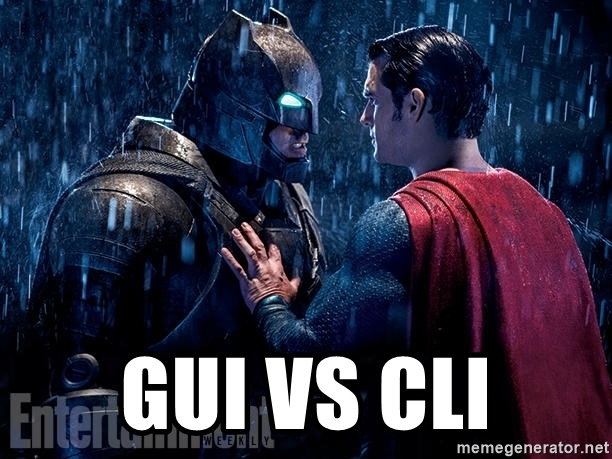
\includegraphics[width=0.7\linewidth]{/Users/statkclee/swc/author_carpentry_kr/tutorial/07_rmarkdown_paper/fig/gui-vs-cli} 

}

\caption{Caption here.}\label{fig:supermanBatman}
\end{figure}

\subsection{수식}

\[\text{생산성} = \frac{\text{CLI}^2}{\text{GUI}}\]

\subsection{표}

\begin{table}

\caption{\label{tab:tableName}Caption here.}
\centering
\begin{tabular}[t]{rr}
\toprule
Plot & sprich\\
\midrule
3294 & 31\\
3297 & 28\\
3299 & 26\\
3330 & 27\\
\bottomrule
\end{tabular}
\end{table}

종족 평균값은 28.

표 참조를 넣은 경우 \ref{t:anova}:

\begin{table}[ht]
\centering
\caption{Caption here} 
\label{t:anova}
\begin{tabular}{lrrrrr}
  \toprule
 & Df & Sum Sq & Mean Sq & F value & Pr($>$F) \\ 
  \midrule
pH          & 1 & 4.58 & 4.58 & 4.77 & 0.2733 \\ 
  shade       & 1 & 8.45 & 8.45 & 8.80 & 0.2070 \\ 
  Residuals   & 1 & 0.96 & 0.96 &  &  \\ 
   \bottomrule
\end{tabular}
\end{table}

수작업으로 표를 넣는 경우 \ref{tab:byhand}:

\begin{longtable}[]{@{}llll@{}}
\caption{\label{tab:byhand} Caption here.}\tabularnewline
\toprule
Col A & Col B & Col C & Col D\tabularnewline
\midrule
\endfirsthead
\toprule
Col A & Col B & Col C & Col D\tabularnewline
\midrule
\endhead
row 1 & 190 & \(112 \pm 2\) & \(233 \pm 3\)\tabularnewline
\(\eta\) & 0.13 & 0.12 & 0.12\tabularnewline
\(\eta^2\) & 0.14 & 0.13 & 0.50\tabularnewline
\(\eta^3\) & 0.15 & 0.31 & 0.52\tabularnewline
\bottomrule
\end{longtable}

\section{R 그래프}\label{r-}

그래프 참조를 하는 방법 \ref{fig:figName}.

\begin{figure}

{\centering 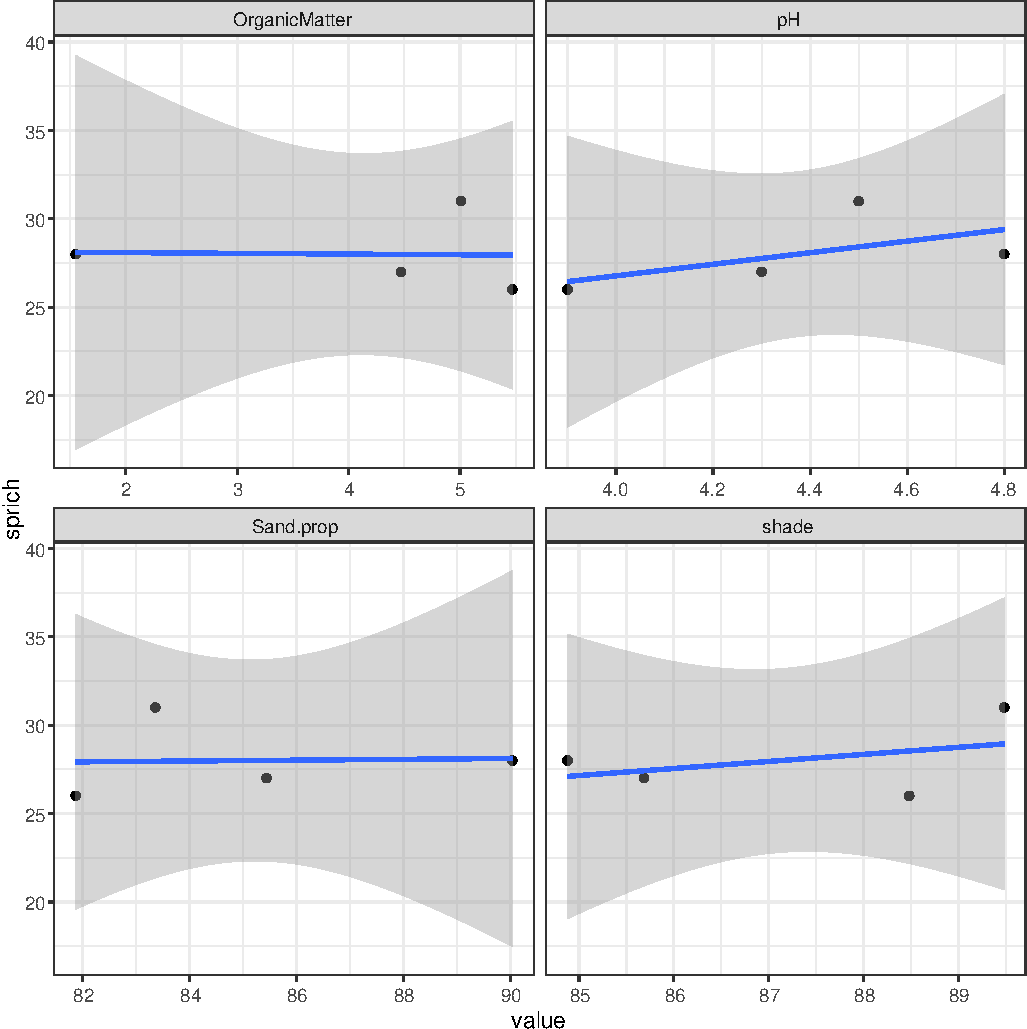
\includegraphics{ms_files/figure-latex/figName-1} 

}

\caption{Your caption here.}\label{fig:figName}
\end{figure}

\subsection{문제해결}

GUI로 해결하기 힘든 아래와 같이 \texttt{pdf} 파일 생성시 생긴 문제는
구글 검색을 통해서 stackoverflow
\href{https://stackoverflow.com/questions/18178084/pandoc-and-foreign-characters}{Pandoc
and foreign characters}에서 해법을 찾아
\texttt{-\/-latex-engine=xelatex\ -V\ CJKmainfont=NanumGothic}와 같이
글꼴까지 반영시킨다.

\begin{verbatim}
! Package inputenc Error: Unicode character 내 (U+B0B4)
(inputenc)                not set up for use with LaTeX.
\end{verbatim}

\section{R 코드}\label{r-}

\subsection{기술통계량}

\begin{verbatim}
##       mpg            cyl            disp           hp           drat     
##  Min.   :10.4   Min.   :4.00   Min.   : 71   Min.   : 52   Min.   :2.76  
##  1st Qu.:15.4   1st Qu.:4.00   1st Qu.:121   1st Qu.: 96   1st Qu.:3.08  
##  Median :19.2   Median :6.00   Median :196   Median :123   Median :3.69  
##  Mean   :20.1   Mean   :6.19   Mean   :231   Mean   :147   Mean   :3.60  
##  3rd Qu.:22.8   3rd Qu.:8.00   3rd Qu.:326   3rd Qu.:180   3rd Qu.:3.92  
##  Max.   :33.9   Max.   :8.00   Max.   :472   Max.   :335   Max.   :4.93
\end{verbatim}

\subsection{회귀모형}

\begin{verbatim}
## # A tibble: 2 x 5
##   term        estimate std.error statistic  p.value
##   <chr>          <dbl>     <dbl>     <dbl>    <dbl>
## 1 (Intercept)  29.6      1.23        24.1  3.58e-21
## 2 disp         -0.0412   0.00471     -8.75 9.38e-10
\end{verbatim}

\subsection{시각화}

\begin{figure}

{\centering 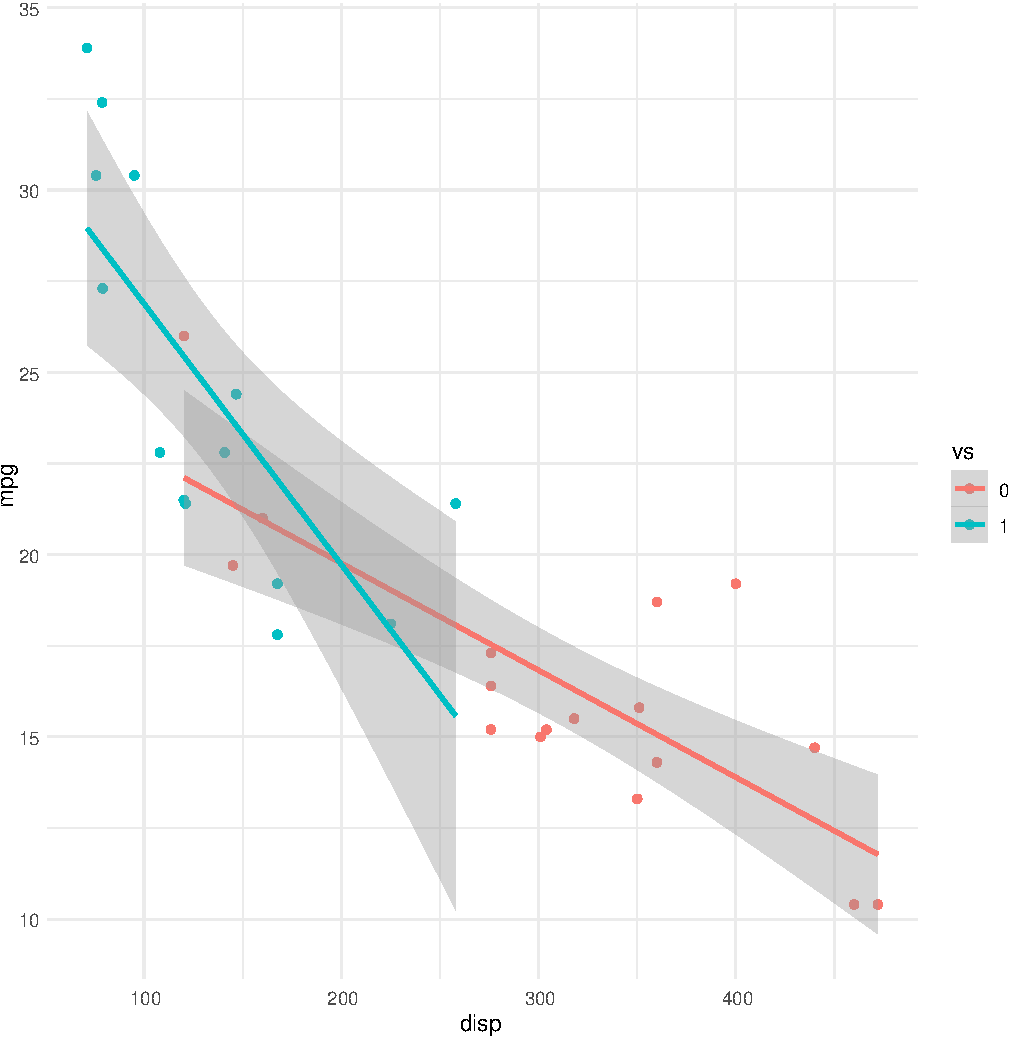
\includegraphics{ms_files/figure-latex/mtcarsGraph-1} 

}

\caption{Mtcars 그래프}\label{fig:mtcarsGraph}
\end{figure}

\subsection{\texorpdfstring{첨부: \texttt{pandoc} 컴파일
코드}{첨부: pandoc 컴파일 코드}}\label{-pandoc--}

\section*{참고문헌}
\addcontentsline{toc}{section}{참고문헌}

\hypertarget{refs}{}
\hypertarget{ref-DBLP:journalsux2fcorrux2fSimperlerW15}{}
\textsc{Simperler, A. and Wilson, G.} 2015. Software carpentry get more
done in less time. \emph{CoRR} \emph{abs/1506.02575}.

\hypertarget{ref-10.1371ux2fjournal.pbio.1001745}{}
\textsc{Wilson, D.A.A.B., Greg AND Aruliah}. 2014. Best practices for
scientific computing. \emph{PLOS Biology} \emph{12}, 1, 1--7.


\end{document}
